\columnbreak
\section{Anlagetypen}

\subsection{Klassifizierung}

\begin{outline}
    \1 Aufdachanlagen
        \2 Schrägdach
    \1 Indachanlagen
    \1 Flachdachanlagen
        \2 Typischerweise Befestigung durch Beschwerung (keine Dachdurchdringung)
            \3 Aerodynamische Systeme
            \3 Flacher Aufbau
            \3 Verbindung der Reihen
        \2 Meist Ost-West-Ausrichtung, ca. 10--15° Neigung
        \2 Aplin
            \3 Vertikal Bifazial
            \3 Solartanne
    \1 Fassadenanlagen
        \2 Herausforderungen:
            \3 Statik (geprüftes Gesamtsystem oder Prüfung im Einzelfall)
            \3 Brandschutz (Brände breiten sich vertikal schneller aus)
            \3 Optik (Farbe, Form, Haptik, Reflexion/Blendung)
            \3 Wartung und Zugänglichkeit Technik
    \1 Freiflächenanlagen
    \1 Weitere / neue Konzepte
        \2 Infrastruktur 
            \3 Parkplatzüberdachung
            \3 Lärmschutzwände
            \3 Staudämme
            \3 Solarfaltdach auf ARA 
        \2 Agri-PV
            \3 Müssen nach Raumplanungsverordnung (RPV) Art. 32c in wenig empfindlichen Gebieten Vorteile für die landwirtschaftliche Produktion bewirken oder entsprechenden Versuchs- und Forschungszwecken dienen.
        \2 Floating-PV
        \2 Fahrzeugintegrierte PV (Vehicle Integrated PV -- VIPV)
        \2 Plug\&Play PV (Stecker-PV)
            \3 Bis 600 W AC-Ausgangsleistung des Wechselrichters
  \end{outline}


\subsection{Bifaziale Module}
Beide Seiten des Moduls zur Stromerzeugung genutzt!\\

\vspace{0.25cm}

\subsubsection{Prinzipschema}
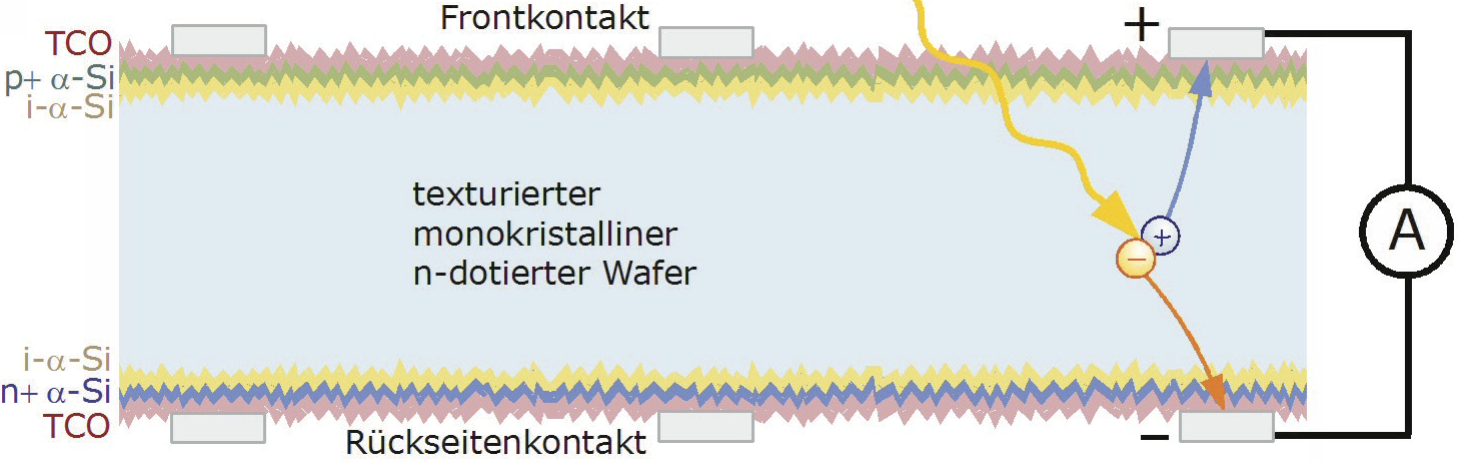
\includegraphics[width=0.95\columnwidth]{images/Bifaziale Module 1.png}

\vspace{0.25cm}

\subsubsection{Funktionsprinzip}
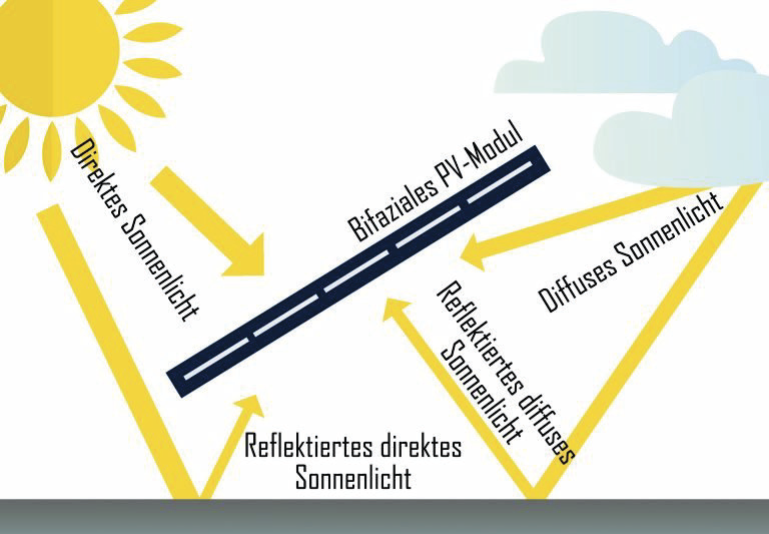
\includegraphics[width=0.5\columnwidth]{images/Bifaziale Module 2.png}

























